\makeatletter
\newenvironment{adjustmargins}[2]{%
 \begin{list}{}{%
 \topsep\z@%
 \listparindent\parindent%
 \parsep\parskip%
 \checkoddpage
 \ifoddpage % odd numbered page
 \@ifmtarg{#1}{\setlength{\leftmargin}{\z@}}%
 {\setlength{\leftmargin}{#1}}%
 \@ifmtarg{#2}{\setlength{\rightmargin}{\z@}}%
 {\setlength{\rightmargin}{#2}}%
 \else % even numbered page
 \@ifmtarg{#2}{\setlength{\leftmargin}{\z@}}%
 {\setlength{\leftmargin}{#2}}%
 \@ifmtarg{#1}{\setlength{\rightmargin}{\z@}}%
 {\setlength{\rightmargin}{#1}}%
\fi
}
\item[]}{\end{list}}

\makeatother


\chapter{Pages}

\parindent1em

The page is the main element in a book and its geometry and layout has been studied extensively by typographers. In this chapter we outline the typographical tradition, methods to specify layouts using \latex and associated issues, such as adjusting margins within a page.

Bringhurst notes that ``much typography is based, for the sake of economy on standard industrial sizes, from $35\times45$ inch press sheets to $3 1/2$ x 2 inch conventional business cards. Some formats as the booklets that accompany mobile telephone kits, are condemned to especially rigid restrictions of size.  

There may already be some restrictions on the page size you choose depending on your method of production and distribution. If you aim to output pages on a desktop printer then a standard size like A4 ($297\times210$)mm or US letter ($11\times 8 1/2$ inches) is advisable. If you have the opportunity and necessity of selecting the dimensions of the page you have a great opportunity to enhance the page layout of your book.

\section{Selecting  paper sizes}

Besides the limitations of the method of printing, another consideration is the size of book you writing and the
audience you are addressing it. If you are only producing a 60 page book, paper with smaller dimensions might be more appropriate than a blockbuster novel. 

History, natural science, geometry and mathematics are all relevant to typography.


\begin{figure}[ht]
\centering
\includegraphics[width=0.5\textwidth]{./images/preparing-paper.jpg}
\caption{Getting paper prepared for printing \protect\cite{moxon}.}
\end{figure}

Originally, paper sizes were determined by the moulds the paper was
made in and the use the result was put to. While many hundreds of variations have occurred throughout the centuries, in the main there have seldom been more than six categories of sizes in use since the fourteenth century. These have often come down to us bearing the names of the figures featured in the paper's watermarks, such as \emph{foolscap},
\emph{elephant}, \emph{pot}, and \emph{crown}. To enable the creation of smaller sizes from
existing larger sizes, the sheets have since the Middle Ages been proportioned
with their sides in the ratio of \(1:\sqrt{2}\). For example, quarto (4to,
formerly 4to) and octavo (8vo, formerly 8vo) sizes are obtained by cutting
or folding standard sizes four and eight times respectively.
Former British paper dimensions still used the old sizes before decimalized
versions replaced them; US dimensions still retain most of these
(untrimmed) paper sizes, in inches. Both are still encountered in specialist and bibliographic work, and in reproducing earlier or foreign formats:


\section{Canonical Layouts}

Typographers derive proportions that naturally occur in nature, and pages that embody
them recur in manuscripts and books from Rennaissance Europe, Tang and Song dynasty
China, early Egypt and ancient Rome.  
These numbers are $\pi=$3.14159\ldots , which is the circumference of a circle whose diameter
is one; $\sqrt{2}=$1.41421\ldots , which is the diagonal of a unit square; 
$e=2.71828$  \ldots ,which is the base of the natural logarithms; and $\phi=1.61803$ \ldots ,a number which is discussed later on. Certain of these proportions appear in he structure of the human body; other appear in musical scales. Indeed, one of the simplest of all systems of 
page proportions is based on the familiar intervals of the diatonic scale. Pages that
embody these basic musical proportions have been in common use in Europe for more than a thousand year.

 \begin{figure}
 \makebox[\textwidth]{\makebox[1.1\textwidth][r]{%
 \unitlength=0.0015\textwidth
 \let\ul\unitlength
	\begin{picture}(184,320)(0,-20)
	\put(0,0){\framebox(184,297){}}
	\put(27,70){\makebox(0,0)[bl]{\color{thegray}\rule{113\ul}{184\ul}}}
	\put(92,-20){\makebox(0,0)[t]{Golden number canonical layout}}
	\color{red}
	\put(92,162){\circle{184}}
	\linethickness{.2pt}
	\multiput(0,297)(1.98918918919,-3.21081081082){93}{\line(184,-297){1}}
	\end{picture}%
 \hfill
	\unitlength0.0015\textwidth
	\let\ul\unitlength
		\begin{picture}(210,330)(0,-20)
		\put(0,0){\framebox(210,297){}}
		\put(25,51){\makebox(0,0)[bl]{\color{thegray}\rule{149\ul}{210\ul}}}
		\put(105,-35){\makebox(0,0)[b]{ISO canonical layout}}
		\color{red}
		\put(105,156){\circle{210}}
		\multiput(0,297)(2.27027027027,-3.21081081082){93}{\line(210,-297){1}}
		\end{picture}%
 \hfill
   \unitlength0.001591\textwidth
   \let\ul=\unitlength
   \begin{picture}(220,330)(0,-20)
   		\put(0,0){\framebox(220,280){}}
   		\put(20.742,33.6){\makebox(0,0)[bl]{\color{thegray}\rule{172.86\ul}{220\ul}}}
   		\put(110,-35){\makebox(0,0)[b]{Letter paper canonical layout}}
   		\color{red}
   		\put(110,143.6){\circle{220}}
		\multiput(0,280)(2.37837837838,-3.02702702703){93}{\line(220,-280){1}}
   \end{picture}
 }}%
 \caption{A right page with the relevant diagonal, the text block and the canonical circle.
 In this figure the important information is the page proportions, not the scale; matter of
 fact the letter paper is 17.6 mm shorter than the A4 paper, but the drawings to the same
 height emphasize the relative proportions of the various page parts. \cite{canonicallayout}}
 \label{fig:canoniclayout}
 \end{figure}
 
The package \pkgname{xlayouts} and also Beccari’s \pkgname{canonical} layouts provide both graphical as well as settings for determining page layouts that approach canonical layouts. In reality modern book design has diverged from these principles. 

\begin{figure}[hb]
\cxset{spread xsteps=9,
          spread scale=0.20,
          spread width=0.5\textwidth}
\centering
\drawcanons
\end{figure}


\begin{figure}
  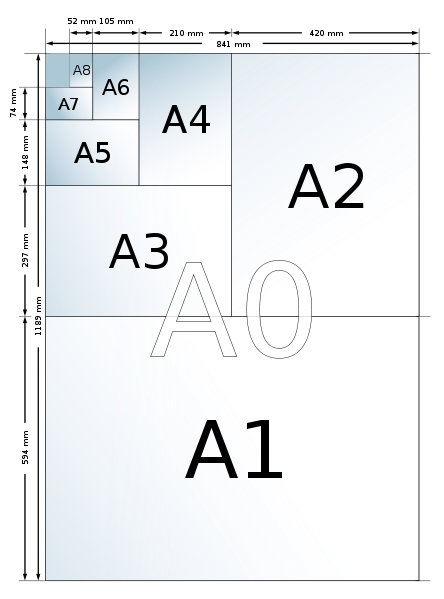
\includegraphics[width=0.5\linewidth]{./graphics/A-sizes.png}
  \caption{When a sheet whose proportions are $1$:$\surd{2}$ is folded in half, the result is a sheet half as large but with \emph{the same proportions}. Standard paper sizes on this principle have been in use in Germany since the early 1920s. The basis of this system is the A0 sheet, which has an are of 1 m$^2$. Yes because it is \textit{reciprocal with nothing but itself}, the ISO page in isolation is the least musical of all the major page shapes. It needs a textblock of another shape or contrast.}
   \label{fig:marginfig1}
\end{figure}

The advantages of basing a paper size upon an aspect ratio of $\surd{2}$ were already noted in 1786 by the German scientist Georg Christoph Lichtenberg, in a letter to Johann Beckmann[2]. The formats that became |A2|, |A3|, |B3|, |B4| and |B5| were developed in France, and published in 1798 during the French Revolution, but were subsequently forgotten. \cite{letimbre2136}

Early in the twentieth century, Dr Walter Porstmann turned Lichtenberg's idea into a proper system of different paper sizes. Porstmann's system was introduced as a DIN standard (DIN 476) in Germany in 1922, replacing a vast variety of other paper formats. Even today the paper sizes are called "DIN Ax" in everyday use in Germany.

The main advantage of this system is its scaling: if a sheet with an aspect ratio of $\surd{2}$ is divided into two equal halves parallel to its shortest sides, then the halves will again have an aspect ratio of $\surd{2}$. Folded brochures of any size can be made by using sheets of the next larger size, e.g. |A4| sheets are folded to make |A5| brochures. The system allows scaling without compromising the aspect ratio from one size to another – as provided by office photocopiers, e.g. enlarging |A4| to |A3| or reducing |A3| to |A4|. Similarly, two sheets of |A4| can be scaled down and fit exactly 1 sheet without any cutoff or margins.

%\cxset{try grid=false}
%\thispagestyle{grid}


The weight of each sheet is also easy to calculate given the basis weight in grams per square metre (g/m² or `'gsm"). Since an |A0| sheet has an area of 1m² , its weight in grams is the same as its basis weight in g/m². A standard |A4| sheet made from 80 g/m² paper weighs 5g, as it is one 16th (four halvings) of an A0 page. Thus the weight, and the associated postage rate, can be easily calculated by counting the number of sheets used.

Unlike the |A4| standard paper, the origin of the dimensions of letter size paper are lost in tradition. The American Forest and Paper Association argues that the dimension originates from the days of manual paper making, and that the 11-inch length of the page is about a quarter of ``the average maximum stretch of an experienced vatman's arms".[1] However, this does not explain the width or aspect ratio. What is known is that Ronald Reagan made this the paper size for U.S. federal forms; previously, the smaller "official" size (8 in × 10½ in or 203.2 mm × 266.7 mm) was used.[1] Letter or US Letter is the most common paper size for office use in the United States and Canada. It is 8$\frac{1}{2}$ by 11 inches (exactly 215.9 mm × 279.4 mm).

\section{The Typearea}

According to \cite{bringhurst2005}, in typography margins must do three things. They must lock the
textblock to the page and lock the facing pages to each other through the force of their proportions. Second, they must frame the textblock in a manner that suits its design. Third, they must protect the textblock, leaving it easy for the reader to see and convenient to handle. 

In most well designed books fifty per cent of the character and integrity of a printed page lies in its letterforms. Much of the other fifty per cent resides in its margins.


\subsection{Readability}

Another aspect that determines the text area, is the readability of the text. Here you need to take into account the readers of your book. For children and older persons a larger type and shorter lines are preferred.

\begin{macro}{\alphabetlength}
The macro |\alphabetlength| prints the length of the alphabet. The length of the alphabet in this text is \alphabetlength. If this is a good choice is debatable, but after all this is just a long document, with many chapters and my aim was to produce a reference and a test document. The macro is defined in the |xlayouts|  package, which is loaded automatically by the |phd| package or class. 
\end{macro}

Traditionally  a line that is approximately 1.4 times the alphabet length is considered good practice. The length of one line of text in this document is \the\textwidth giving a ratio of \alphabetsperline.

\DescribeMacro{\printreadability} prints a small table with some readability figures. If LuaTeX is used, this table is slightly longer and prints some other statistics as well. 

\begin{figure}[htbp]
\drawtriallayout
\bigskip

\printreadability
\captionof{figure}{Page layout diagram and readability statistics (using the \pkgname{xlayouts} package).}
\end{figure}

The macros described above are loaded by the |xlayouts| package, which forms part of the |phd| budle. There are macros for drawing trial layouts 


\section{Examples}
Folowing the nomenclature introduced b Bringhurst in analyzing the examples on the following pages, 
these symbols are used:

%% Align at the = sign 
\begin{table}[htbp]
\begin{tabular}{l l @{ = } p{6cm}}
\textit{Proportions:}      &P  &  page proportion $h/w$\\
~                      &T &  textblock proportion: $d/m$\\
\textit{Page size:}         &w &  width of page (trim-size)\\
~                      &h  & height of page (trim-size)\\
\textit{Textblock:}           &m & measure (width of primary textblock)\\
~                      &d  & depth of primary textblock (excluding running heads, folios etc)\\                      
~                      &$\lambda$ & line height (type size plus added lead)\\
~                      &$n$ & secondary measure (width of secondary column)\\
~                      &$c$  & column width, where there are even multiple columns\\
\textit{Margins}  &$s$  & spine margin (back margin)\\
~                      &$t$   & top margin (header margin)\\
                        &$e$  & fore-edge (front margin)\\
                        &$f$   & foot margin\\
                        &$g$  & internal gutter (on a multiple-column page)\\
\end{tabular}
\caption{Symbols used to demonstrate various ratios in books}
\end{table}
\medskip

\begin{figure}
  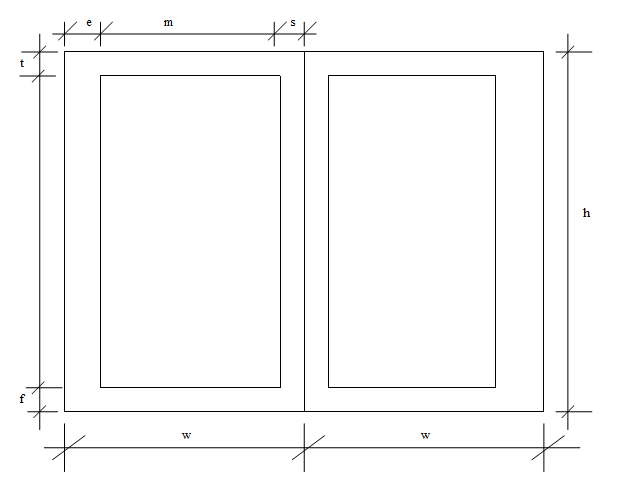
\includegraphics[width=\linewidth]{./graphics/page.png}
  \caption{Page nomenclature}
   \label{fig:marginfig1}
\end{figure}

More variables are necessary to specify all the variables handled by a \latex\
page. For the time being the examples refer to dimensions from historical works
in typography and should sufffice.

\subsection{Hypneroto}

\begin{figure}[htbp]
\centering
  \includegraphics[width=\linewidth]{./graphics/hypneroto.jpg}
\caption{The work is lauded for the originality of its
design. Several sequential double page
illustrations add a visual dimension to the
progression of the narrative, and act like an
early form of the strip cartoon. There is an
obsession with movement throughout which is driven
on by the illustrations, resulting in the
impression of bodies moving from one page to the
next. Other typographical innovations include
playing with the traditional layout of the text;
in the opening shown here, for example, the pages
are shaped in the form of goblets. The dimensions
of the text are: $P=1.5[2:3]$; T=1.7 (tall pentagon);
Margins: s=t=w/9; e=2 s. The text is a fantasy
novel, Francesco Colonna's Hypnerotomachia
Poliphili, set in a roman font cut by Francesco
Griffo. (Aldus Manutius, Venice, 1499). Original
size: $20.5\times31$\thinspace cm.}
\label{fig:hypneroto}
\end{figure}


%  \label{fig:layout}



The book was printed by Aldus Manutius in Venice in December 1499. The book is anonymous, but an acrostic formed by the first, elaborately decorated letter in each chapter in the original Italian reads \textsc{\small POLIAM FRATER FRANCISCVS COLVMNA PERAMAVIT}, \enquote{Brother Francesco Colonna has dearly loved Polia.} However, the book has also been attributed to Leon Battista Alberti by several scholars, and earlier, to Lorenzo de Medici. The latest contribution in this respect was the attribution to Aldus Manutius, and arguably, a Francesco Colonna, a wealthy Roman Governor. The author of the illustrations is even less certain, but contemporary opinion gives the work to Benedetto Bordone.

\section{Contemporary book layouts}

All these sound mystical with religious undertones, but we need to remember that early printers made their livelihoods from printing mostly religious books.

From the mystics to the modern, let us study Figure~\ref{fig:nudes}

\begin{figure}[htbp]
\centering

\fbox{\includegraphics[width=\linewidth]{nudes.jpg}}

\caption{In this layout, the placement of various size images on the right pages, makes the margins disappear to the eye. As the whole book, is made of similar pages\ldots }
\end{figure}

Modern designers are more cryptic. One book that I found more useful is Ambrose/Harris \textit{Layout}. The book brings together examples of layout, both contemporary  and historic, from aroudnd the world. It contains examples from leading graphic designers to provide a sample of rich and diverse possibilities for the creative use of layout.

As it will become apparent from what follows, although at first look it appears that all design principles have disappeared into post modern designs, all design is undertaken with reference to a certain set of principles, either by consciously
choosing to follow or by deliberately ignoring or subverting them. The collective body of principles represents different approaches to design and layout construction.

The principles in this section have been used
through the ages to produce designs that are
pleasing to the eye and that organise information
clearly and efficiently, two of the challenges facing
every graphic designer. These principles affect
decisions made at the heart of the design process,
as they provide the basis of how space is divided.

\section{A design must capture the spirit of the times.}

The word \emph{zeitgeist} originates from the German zeit (time) and geist (spirit),
and so literally means spirit of the age. In graphic design, each decade can
be defined by several predominant zeitgeists that somehow seem to capture
their essence. Today, in graphic design, we can see a zeitgeist for the use of
sophisticated computer graphics giving a very close approximation to reality
in addition to another, which is a backlash to this, in the form of rough-and-ready
hand-drawn designs.

\section{Objects on a Page}

How an object is placed on a page has a dramatic
impact on how it is received and interpreted by
the viewer, and the message that it delivers. We
have looked at how grids can be used to guide
element placement on a page, but maintaining a
sense of order is not the only consideration when
laying out a design.

Object placement helps form the narrative of
a design and is constructed from an understanding
of how we read a page. The narrative of a design
can be created and altered by a wide range of
placement and intervention strategies, such as
how white space is used, the balance and relative
weight given to other objects, the juxtaposition or
contrast of objects and so on.

This chapter will outline some of the
fundamental approaches to object placement.

\section{White Space}

White space is not necessarily white, as it refers to any space in the design
without text or graphic elements. Designers naturally insert white space into
their designs to help the composition and make the information the design
contains easier to access, such as leaving margins at the sides of the page that
create space around text blocks. Swiss typographer Jan Tschichold called white
space ‘the lungs of a good design’. Without white space, with every part of the
design area filled, there is a danger that a design would look cramped and
difficult to understand.

White space can instil different perceptions in a viewer depending on how it is
used and the content it is associated with. White space may give the impression
of luxury and extravagance for a full-page photograph. However, it may also give
the impression that there are gaps in a layout that is rather full, or worse, that
there is insufficient content to fill a page. Newspapers try to establish a rational
balance between giving space to page elements to meet the conflicting demands
of the need for typographical sensitivity and readability, while filling a page with
news so that the reader feels they are getting value for money. Habitually readers
expect a newspaper to be ‘full’, which means it is harder to achieve typographic
balance. In contrast, where filling space is of less concern, such as the example
below, white space becomes a more overt part of the design.



\section{Grids}

\subsection{The Baseline Grid}

The baseline grid is the (invisble) graphic foundation upon which a design is constructed and provides a visual guide for positioning and ligning page elements with an accuracy that is difficult to achieve by eye alone. Knuth's TeX focuses almost primarily on getting this one right.

\section{Pace}

It came to me as a big surprise that a books layout must have \textit{pace}. This essentially is the alternation of pages, between say images and text.

\begin{figure}[htbp]
\parindent=0pt
\includegraphics[width=\textwidth]{pace}

\end{figure}

Thumbnails are smaller versions of the spreads of a publication presented on a
page that allow a designer to gauge its pace and balance at the macro level
without focusing on details. Thumbnails allow a designer to look at the
narrative of the publication and tune it as a whole, rather than on a spread-byspread
basis.

Pictured are thumbnails for Miss X, a book for underwear retailer Agent
Provocateur art directed by Mike Figgis and published by Anova, with design by
Gavin Ambrose. The absence of folios and minimal text mean the image flow
takes prominence.

The images can let us set a method for defining such spreads. 


\chapter{Temporarily changing the text width}

\index{pagewidth>change temporarily}


Margins in a page can be changed temporarily by adjusting, the lengths of \cmd{\leftskip} and \cmd{\rightskip}. The |memoir| class provides an environment |adjustwidth| see page 422 (based on This code is based on the \pkgname{chngpage} package.) for doing so and the \class{tufte-book} class provides an environment \textit{fullwidth}. The following code is an adaptation of that found in the \class{memoir} class.


\begin{teXX}
\begin{adjustmargins}{left}{right} 
\end{teXX}


adds the given lengths to the left and
right hand margins. A positive value will shorten the text and a negative value
will widen it. The starred version of the environment will cause the margin changes to switch between odd and even pages. 



\eject
\newgeometry{left=10mm,right=10mm,bottom=1.5cm,top=1cm}

\section*{The \texttt{adjustmargins} environment}
\lorem

\vfill\vfill
\begin{multicols}{2}
\lorem
\end{multicols}

\begin{adjustmargins}{0cm}{0in}
{\leftskip1em\rule{13cm}{.4pt}\par}

\centering



\parbox{\textwidth}{{\leftskip1em\rightskip1em There are no engineers in the hottest parts of hell, because the existence of a 'hottest part' implies a temperature difference, and any marginally competent engineer would immediately use this to run a heat engine and make some other part of hell comfortably cool.  This is obviously impossible.\par}
}
\par
\medskip
\par
\noindent\includegraphics[width=0.9\textwidth]{./graphics/lilian.jpg}\par


\end{adjustmargins}

\clearpage

\restoregeometry


\lipsum[1]


\begin{adjustmargins}{-0.4\textwidth}{0.1\textwidth}
\fboxsep2pt%
\fbox{\includegraphics[width=1.2\textwidth]{./graphics/leoncroll.jpg}}
\end{adjustmargins}

\lipsum[2]

\begin{teX}
\begingroup
\makeatletter
 \catcode`\Q=3
 \long\gdef\@ifmtarg#1{\@xifmtarg#1QQ\@secondoftwo\@firstoftwo\@nil}
 \long\gdef\@xifmtarg#1#2Q#3#4#5\@nil{#4}
 \long\gdef\@ifnotmtarg#1{\@xifmtarg#1QQ\@firstofone\@gobble\@nil}
 \endgroup


\newenvironment{adjustmargins}[2]{%
  \begin{list}{}{%
    \topsep\z@%
    \listparindent\parindent%
    \parsep\parskip%
   \@ifmtarg{#1}{\setlength{\leftmargin}{\z@}}%
   {\setlength{\leftmargin}{#1}}%
   \@ifmtarg{#2}{\setlength{\rightmargin}{\z@}}%
   {\setlength{\rightmargin}{#2}}%
}
\item[]}{\end{list}}
\makeatother
\end{teX}

 
\section{Setting Dimensions in \latex}

To set dimensions for page layout in \latex is not straightforward. You need to adjust several \latex
native dimensions to place a text area where you want. If you want to center the text area in the paper
you use, for example, you have to specify native dimensions as follows:

\begin{verbatim}
\usepackage{calc}
\setlength\textwidth{7in}
\setlength\textheight{10in}
\setlength\oddsidemargin{(\paperwidth-\textwidth)/2 - 1in}
\setlength\topmargin{(\paperheight-\textheight
-\headheight-\headsep-\footskip)/2 - 1in}.
\end{verbatim}

Without package |calc|, the above example would need more tedious settings. To adjust all parameters from scratch one should have a good understanding, of \latexe's definitions of all parameters. The companion package |xlayouts| can be used to display these parameters on an actual printed page. All settings are parameterized and I find the use of colours assists in viewing the rulers better.


\subsection{The Geometry package}

The package \pkg{geometry} \cite{geometry} provides
an easy way to set page layout parameters. In this case, what you have to do is just load the package and set
the page geometry using keys.

\begin{teX}
\usepackage[text={7in,10in},centering]{geometry}.
\end{teX}

Besides centering problem, setting margins from each edge of the paper is also troublesome. But geometry
also make it easy. If you want to set each margin to 1.5in, you can type

\begin{comment}
\label{sec:geometry}

\def\OpenB{{\ttfamily\char`\{}}
 \def\Comma{{\ttfamily\char`,}}
 \def\CloseB{{\ttfamily\char`\}}}
 \def\Gm{\textsf{geometry}}
\newcommand\gpart[1]{\textsf{\textsl{\color[rgb]{.0,.45,.7}#1}}}%

\newcommand\glen[1]{\textsf{#1}}

\bgroup
\makeatletter
 \begin{figure}
  \small
  \unitlength=.65pt
  \begin{picture}(450,250)(0,-10)
  \put(20,0){\framebox(170,230){}}
  \put(20,235){\makebox(170,230)[br]{\gpart{paper}}}
  \begingroup\thicklines
  \put(40,30){\framebox(120,170){}}
  \put(40,30){\makebox(120,165)[tr]{\gpart{total body}~}}
  \put(45,30){\makebox(0,170)[l]{|height|}}
  \put(40,35){\makebox(120,0)[bc]{|width|}}
  \put(50,-20){\makebox(120,0)[bc]{|paperwidth|}}
  \put(10,45){\makebox(0,170)[r]{|paperheight|}}
  \put(90,200){\makebox(0,30)[lc]{|top|}}
  \put(90,0){\makebox(0,30)[lc]{|bottom|}}
  \put(10,70){\makebox(0,0)[r]{|left|}}
  \put(10,55){\makebox(0,0)[r]{(|inner|)}}
  \put(200,70){\makebox(0,0)[l]{|right|}}
  \put(200,55){\makebox(0,0)[l]{(|outer|)}}
  \put(80,230){\vector(0,-1){30}}\put(80,30){\vector(0,-1){30}}
  \put(80,200){\vector(0,1){30}}\put(80,0){\vector(0,1){30}}
  \put(20,70){\vector(1,0){20}}\put(40,70){\vector(-1,0){20}}
  \put(160,70){\vector(1,0){30}}\put(190,70){\vector(-1,0){30}}
  \multiput(160,30)(5,0){24}{\line(1,0){2}}
  \multiput(160,200)(5,0){24}{\line(1,0){2}}
  \begingroup\thicklines
  \put(280,30){\framebox(120,170){}}\endgroup
  \put(283,133){\makebox(0,12)[l]{|textheight|}}
  \put(295,130){\vector(0,-1){100}}\put(295,150){\vector(0,1){50}}
  \multiput(280,220)(5,0){24}{\line(1,0){3}}
  \put(280,208){\makebox(120,20)[bc]{\gpart{head}}}
  \multiput(280,207)(5,0){24}{\line(1,0){3}}
  \put(420,225){\makebox(0,0)[l]{|headheight|}}
  \put(418,225){\line(-2,-1){20}}
  \put(420,213){\makebox(0,0)[l]{|headsep|}}
  \put(418,213){\line(-2,-1){20}}
  \put(420,12){\makebox(0,0)[l]{|footskip|}}
  \put(418,12){\line(-2,1){20}}
  \put(280,40){\makebox(120,140)[c]{\gpart{body}}}
  \put(305,45){\vector(-1,0){25}}\put(375,45){\vector(1,0){25}}
  \put(80,230){\vector(0,-1){30}}\put(80,30){\vector(0,-1){30}}
  \put(280,48){\makebox(120,0)[c]{|textwidth|}}
  \put(280,15){\makebox(120,10)[c]{\gpart{foot}}}
  \multiput(280,14)(5,0){24}{\line(1,0){2}}
  \put(410,30){\dashbox{3}(30,170){}}
  \put(415,30){\makebox(30,170)[l]{\gpart{marginal note}}}
  \put(425,45){\vector(-1,0){15}}\put(425,45){\vector(1,0){15}}
  \put(450,70){\makebox(0,0)[l]{|marginparsep|}}
  \put(448,70){\line(-3,-1){43}}
  \put(450,45){\makebox(0,0)[l]{|marginparwidth|}}
  \end{picture}
\caption{Dimension names used in the geometry package. width $=$ textwidth and height $=$ textheight by default. left, right, top and bottom are margins. If margins on verso pages are swapped by twoside option, margins specified by left and right options are used for the inside and outside margins respectively. inner and outer are aliases of left and right
respectively.}
\label{fig:geometrylayout}
\end{figure}
\makeatother
\egroup
\end{comment}

 The \pkg{geometry} package provides a flexible and easy interface to page dimensions.
 You can change the page layout with intuitive parameters. For instance,
 if you want to set a margin to 2cm from each edge of the paper,
 you can type just |\usepackage[margin=2cm]{geometry}|. 
 The page layout can be changed in the middle of the document
 with \cs{newgeometry} command.  The \ref{fig:geometrylayout}, reproduced from the package documentation, illustrates the variety of parameters that can be set using the package.


\section{Footnotes}
The history of footnotes is as long and complicated as the history of scholarship and commentary. Hebrew scholars more than two thousand years ago used systems of glossing and annotation to work on religious texts. 

Scribes in the Christian tradition in the medieval period made use of annotations in their manuscript copying practices: surrounding the original text with glosses in small letters. After the advent of printing, similar kinds of marginal annotation appeared in printed texts of the late fifteenth century. 

Humanist scholars producing printed editions of classical learning in the sixteenth century also made use of the resources of typography to display both the surviving classical text and their commentary on the same page. References to classical sources - and to modern printed editions - became more systematic, as did the expectation that such references would be consistent with scholarly practices. Scholars increasingly marked their professionalism by using complex citational conventions, which by the seventeenth century were so well established as to be the subject of parody and satire. Scriblerian satire of the early eighteenth century, whose purpose was to mock the pedantry and folly of the works of the learned, frequently included extensive parodies of footnotes and the scholarly contests they encoded. Nonetheless, during the eighteenth century, to appear authoritative and learned an author had to adopt the scholarly machinery of the reference citation.

The footnote was born out of a desire to rationalise the relation between text and citation. 

Robert Connors argues that marginal notations fell out of favour for two practical reasons: they left too much blank paper at the side of the text; and they were difficult for typographers to set. The same notes placed at the bottom of the page were more efficient, both in paper and time[1]. 

Anthony Grafton's The Footnote: A Curious History suggests the modern footnote, inaugurated by Pierre Bayle's Dictionaire Critique et Historique in 1697, signalled an epistemic revolution in historical scholarship, indicating the end of credulous scholasticism and the emergence of analytical historical methodologies. Both scholars note the considerable impact of historians such as David Hume and Edward Gibbon on the stylistic development of the discursive and citational footnote as a location for the display of gentlemanly ease as much as scholarly acumen. In the nineteenth century, German scholars such as Leopold von Ranke and Alexander von Humboldt established a systematic basis for the footnote citation, creating a methodical methodological approach that all competing scholars had to obey. In this way, the idea of the footnote was established, yet no there was no general agreement on the form these footnotes should adopt. A systematic approach to the form of the footnote was needed.

In this section we will discuss how lines and paragraphs are turned into pages and how elements of pages such as footnotes, headers etc are inserted. As with the other chapters we will mix TeX basic commands with the more convenient \LaTeXe\ commnads. We will also look at some of the packages and classes that are availble to assist us with page layouts. 


Besides illustrations that are inserted at the top of a page, plain TEX will also
insert footnotes at the bottom of a page. The ootnote macro is provided
for use within paragraphs;  for example, the footnote in the present sentence was typed
in the following way:


There are two parameters to a footnote[ first comes the reference mark, which will
appear both in the paragraph** and in the footnote itself, and then comes the text of
the footnote.45 The latter text may be several paragraphs long, and it may contain
\footnote{Sidenote: ``Where God meant footnotes to go.'' ---Tufte}

\marginpar{

The history of footnotes is as long and complicated as the history of scholarship and commentary. Hebrew scholars more than two thousand years ago used systems of glossing and annotation to work on religious texts. Scribes in the Christian tradition in the medieval period made use of annotations in their manuscript copying practices: surrounding the original text with glosses in small letters. After the advent of printing, similar kinds of marginal annotation appeared in printed texts of the late fifteenth century. Humanist scholars producing printed editions of classical learning in the sixteenth century also made use of the resources of typography to display both the surviving classical text and their commentary on the same page. References to classical sources - and to modern printed editions - became more systematic, as did the expectation that such references would be consistent with scholarly practices. Scholars increasingly marked their professionalism by using complex citational conventions, which by the seventeenth century were so well established as to be the subject of parody and satire. Scriblerian satire of the early eighteenth century, whose purpose was to mock the pedantry and folly of the works of the learned, frequently included extensive parodies of footnotes and the scholarly contests they encoded. Nonetheless, during the eighteenth century, to appear authoritative and learned an author had to adopt the scholarly machinery of the reference citation.

The footnote was born out of a desire to rationalise the relation between text and citation. Robert Connors argues that marginal notations fell out of favour for two practical reasons: they left too much blank paper at the side of the text; and they were difficult for typographers to set. The same notes placed at the bottom of the page were more efficient, both in paper and time[1]. Anthony Grafton's The Footnote: A Curious History suggests the modern footnote, inaugurated by Pierre Bayle's Dictionaire Critique et Historique in 1697, signalled an epistemic revolution in historical scholarship, indicating the end of credulous scholasticism and the emergence of analytical historical methodologies. Both scholars note the considerable impact of historians such as David Hume and Edward Gibbon on the stylistic development of the discursive and citational footnote as a location for the display of gentlemanly ease as much as scholarly acumen. In the nineteenth century, German scholars such as Leopold von Ranke and Alexander von Humboldt established a systematic basis for the footnote citation, creating a methodical methodological approach that all competing scholars had to obey. In this way, the idea of the footnote was established, yet no there was no general agreement on the form these footnotes should adopt. A systematic approach to the form of the footnote was needed.}

Further reading:

Connors, Robert J., 'The Rhetoric of Citation Systems, Part I: The Development of Annotation Structures from the Renaissance to 1900', Rhetoric Review, 17 (1998), 6-48.

Connors, Robert J., 'The Rhetoric of Citation Systems, Part II: Competing Epistemic Values in Citation', Rhetoric Review, 17 (1999), 219-245.

Grafton, Anthony, The Footnote: A Curious History (London: Faber and Faber, 1997)

Grafton, Anthony, 'The Footnote from De Thou to Ranke', History and Theory, 33 (1994), 53-76

Zerby, Chuck, The Devil's Details: A History of Footnotes (Lancaster: Gazelle, 2002)

[1] Robert J. Connors, The Rhetoric of Citation Systems, Part I: The Development of Annotation Structures from the Renaissance to 1900, Rhetoric Review, 17 (1998), 6-48 (p. 30).
